\documentclass[../../main.tex]{subfiles}

\begin{document}

\chapter{Foundations and Models}

\section{The do-it-all Hamiltonian}

In the realm of solid state physics, the many-body Schrödinger equation plays a crucial role in understanding the behaviour of electrons in crystalline materials. This equation provides a fundamental framework for describing the quantum mechanical interactions between multiple electrons within a solid. The Schrödinger Hamiltonian for a system consisting of $N_{\text{el}}$ electrons and $N_{\text{ion}}$ atomic cores --- in its full beauty --- reads
\begin{align}\label{eq:hamiltonian_full}
        \mathcal{H}&=-\frac{\hbar^2}{2M}\sum_{i}^{N_{\text{ion}}}\nabla^2_{\vv{R}_i}-\frac{\hbar^2}{2m}\sum_{i}^{N_{\text{el}}}\nabla^2_{\vv{r}_i}+\frac{1}{2}\sum_{i\neq j}^{N_{\text{ion}}}\frac{Z_i Z_j e^2}{|\vv{R}_i-\vv{R}_j|}+\nonumber\\
        &\qquad\qquad+\frac{1}{2}\sum_{i\neq j}^{N_{\text{el}}}\frac{e^2}{|\vv{r}_i-\vv{r}_j|}-\sum_i^{N_{\text{el}}}\sum_j^{N_{\text{ion}}}\frac{Z_j e^2}{|\vv{r}_i-\vv{R}_j|}+\mathcal{V}_R,  
\end{align}
where $\vv{r}_i$ ($\vv{R}_i$) are the positions of the electrons (ions), $m$ ($M$) their respective masses and $Z_i$ the atomic number of the cores from which the crystal is constructed. The Hamiltonian above can be described in a very simple manner: the first two terms describe the kinetic energy of the ions and electrons, whereas the third and fourth terms denote the mutual Coulomb interaction between all ions and electrons. The second to last term corresponds to the coupling between the ions and electrons and finally $\mathcal{V}_R$ expresses any relativistic effects\footnote{e.g., spin-orbit coupling, relativistic mass correction, anomalous magnetic moments, relativistic Doppler shifts, Zitterbewegung, etc. An instructive example are the relativistic effects that take place in mercury: The binding orbitals of mercury are Lorentz-contracted due to the high speed of the electrons inside these orbitals. This results in a reduction in bonding strength, where ultimately mercury is forming a liquid at room temperatures. In most real solids however, relativistic effects are always negligible and this term will not play a significant role in the majority of calculations.}. The \say{only} thing left to do is solve the Schrödinger equation using the Hamiltonian of \eqref{eq:hamiltonian_full}
\begin{align}
	\mathcal{H}\psi(\{\vv{r}_i\},\{\vv{R}_i\})=E\psi(\{\vv{r}_i\},\{\vv{R}_i\}),
\end{align}
which is easier said than done. The primary problem one faces by trying to do exactly that is the sheer number of particles present in a crystalline material. To be more precise, the wavefunction needed to fulfil the eigenvalue equation above would have to depend on all the degrees of freedom of $\mathcal{O}(10^{23})$ electrons and atoms present in solids. The exponential growth in the number of configurations makes it computationally infeasible to directly calculate or even store this quantity, and already a very small number of electrons and atoms $\mathcal{O}(10)$ exceeds the capability of most modern supercomputers. Thus, one goal of condensed matter physicists is not to find the underlying original Hamiltonian but instead to construct approximate models that contain all the physics necessary while still being controllable and numerically feasible.

Usually, approaches to approximate \eqref{eq:hamiltonian_full} fall into two main categories: (i) using approximate methods to solve the exact Hamiltonian, or (ii) applying (more) exact methods to solve an approximate, mathematically simpler Hamiltonian. Density functional theory (DFT), as an example, falls under the first category, whereas dynamical mean-field theory (DMFT) or the dynamical vertex approximation ($\text{D}\Gamma\text{A}$) reside in category two. The latter build upon a model Hamiltonian which usually incorporates only a subset of all degrees of freedom, e.g., specific orbitals of atomic shells. In modern calculations, a combination of different tools is used to calculate physical properties of materials. For example, a DFT calculation provides a band structure, where the most relevant orbitals are picked, wherefrom more sophisticated methods, such as DMFT or $\text{D}\Gamma\text{A}$ can be applied. Within this thesis, we mainly focus on the method of dynamical vertex approximation, however, we will give a short introduction to DFT and DMFT later to complete the spectrum. 

\section{The Born-Oppenheimer approximation}

Almost a century ago it was caught that the timescales of the electronic and ionic systems are tremendously different due to their large difference in masses. An electron is around a factor 1800 lighter than a proton. Cores in real solids that contain, e.g., transition metal elements, are five orders of magnitude heavier than electrons. Since relaxation time scales inversely with mass, the electrons usually relax in a much shorter time frame than the ionic cores do, hence one can treat them to be always in the equilibrium position as the cores move through the lattice. This allows us, to a very good approximation, to solve the electronic degrees of freedom for static ionic coordinates. This approximation, called the Born-Oppenheimer approximation, is highly useful in condensed matter physics since it enables the study of electronic band structures, energy levels, and transport properties without the need to explicitly account for the complex interactions between electrons and lattice vibrations induced by the motion of ionic cores. However there are certain phenomena, e.g., conventional phonon-mediated superconductivity, where the coupling of lattice vibrations with electrons can not be neglected. However, there are methods, like perturbation theory, which allow to circumvent this apparent issue. Within the regime of the Born-Oppenheimer approximation, the Hamiltonian of \eqref{eq:hamiltonian_full} reduces to
\begin{align}\label{eq:hamiltonian_born_oppenheimer}
	\mathcal{H}_{\text{B-O}}=-\frac{\hbar^2}{2m}\sum_i^{N_{\text{el}}} \nabla^2_{\vv{r}_i}+\frac 12\sum_{i\neq j}^{N_{\text{el}}} \frac{1}{|\vv{r}_i-\vv{r}_j|}+\sum_i^{N_{\text{el}}}\mathcal{V}_{\text{ext}}(\vv{r}_i),
\end{align}
where $\mathcal{V}_{\text{ext}}$ describes any external potential, e.g., from ions of the lattice. The other quantities appearing in \eqref{eq:hamiltonian_born_oppenheimer} have already been introduced in \eqref{eq:hamiltonian_full}. This approximation will serve as the basis for all upcoming models if not stated otherwise.

Despite this large simplification, the eigenvalues and the wavefunctions of the Hamiltonian in \eqref{eq:hamiltonian_born_oppenheimer} are still impossible to compute for real-world solids. Most of the difficulties lie in the second term of \eqref{eq:hamiltonian_born_oppenheimer}, which describes the Coulomb interaction between pairs of electrons. Due to this mutual electromagnetic interaction, the evolution of every electron is influenced by all other electrons present. Hence all electrons are correlated with each other. In general, these effects are of course not negligible, however in some materials\footnote{E.g. for most metals.}, where the electrons are very mobile, screening effects take place which weaken the Coulomb interaction between the electrons. In this context, a very successful ansatz to make \eqref{eq:hamiltonian_born_oppenheimer} treatable is to model the system as electrons interacting with an effective mean-field generated by all other electrons in its proximity. Such a mean field approach is density functional theory. 

\section{Density functional theory}\label{sec:dft}

The basic idea of density functional theory (DFT) is to work with a simple quantity, i.e., the electron density $\rho(\vv{r})$, instead of trying to solve the ab-initio Hamiltonian of \eqref{eq:hamiltonian_born_oppenheimer} - or other, mathematically simpler variants - through complicated many-body wavefunctions. This is possible, at least for the ground state energy and its derivatives, thanks to the two Hohenberg-Kohn theorems, which in essence state that (i) the ground state energy is a unique functional of the electron density $E[\rho(\vv{r})]$ (ii) which is minimized at the ground state density $\rho(\vv{r})=\rho_0(\vv{r})$. This looks already quite promising, however, DFT lacks in some aspects: firstly, the two H-K theorems do not suggest any constructive/mathematical way to obtain the energy functional; secondly, this only holds for the ground state density. There is no way to extract any information from excited states; and lastly, the $3N$-dimensional object $\psi(\{\vv{r}_i\})$ is compressed into a three-dimensional object $\rho(\vv{r})$. Consequently, an arbitrarily tiny variation in $\rho(\vv{r})$ might correspond to a huge change in $E[\rho(\vv{r})]$.

The big question is: \say{How does one approximate the energy functional $E[\rho(\vv{r})]$?}. To answer this, we start with splitting up the energy functional to distinguish different contributions,
\begin{align}
	E[\rho(\vv{r})]=T[\rho(\vv{r})]+E_{\text{H}}[\rho(\vv{r})]+\integral{}{}{^3r}\rho(\vv{r})\mathcal{V}(\vv{r})+E_{\text{XC}}[\rho(\vv{r})].
\end{align}
Here, $T[\rho(\vv{r})]$ denotes the kinetic energy of the electrons. Computing the kinetic energy functional often turns out to be very challenging. $E_{\text{H}}[\rho(\vv{r})]$ is the electrostatic energy (inter alia self-interaction of electrons), given by the Hartree-term
\begin{align}
	E_{\text{H}}[\rho(\vv{r})]=\frac 12\integral{}{}{^3r}\integral{}{}{^3r'}\frac{\rho(\vv{r})\rho(\vv{r}')}{|\vv{r}-\vv{r}'|}.
\end{align}
The potential term includes energies of electrons in external potentials (e.g., nuclei) and is usually not hard to calculate. Lastly, $E_{\text{XC}}[\rho(\vv{r})]$ includes everything else, i.e., the exchange and correlation energies. Dealing with the potential and the Hartree-term is easy compared to the treatment of the kinetic and exchange/correlation functional. There are many ways to construct the kinetic and XC functionals. The most frequently used framework to include the main contribution to the kinetic energy functional is Kohn-Sham DFT and exchange/correlation functionals can be obtained by the local density approximation (LDA) or higher-order variants within K-S DFT, such as different flavours of generalized gradient approximations (GGA). Stepping higher on Jacob's ladder\footnote{Refers to a hierarchical classification of density functional approximations (DFAs) used in Kohn-Sham density functional theory (DFT). The ladder represents a sequence of increasingly accurate and complex approximations for the exchange-correlation energy, which is a key component of the total energy in DFT. Jacob's Ladder begins with the simplest and least accurate approximations at the lower rungs and progresses towards more sophisticated and accurate methods at the higher rungs. Each rung represents a level of approximation that includes additional physical effects and improves upon the previous level.}, more sophisticated methods are hyper-GGA or several variants of (range-separated) hybrid functionals.

This already sounds very promising, why should we not stop here and solely describe our metals with DFT? This apparent question can be answered very straightforwardly: increased localization of $d$ or $f$ orbitals and increased correlation effects therein. Since orbitals with higher angular momentum are more localized in real space, electronic densities in those orbitals are higher and consequently, the electrons within those orbitals are more correlated. Consequently, screening of other itinerant electrons is, in a way, suppressed. Therefore, since DFT is a mean-field approach and relies on the concept of screening, it is not very successful in describing those systems. For example, DFT predicts a metallic behaviour in partially filled $3d$ transition metal or $4f$ rare-earth elements, whereas experiments find them to be insulating. Thus, for strongly correlated materials, sophisticated many-body methods, which do not approximate the Born-Oppenheimer Hamiltonian of \eqref{eq:hamiltonian_born_oppenheimer}, are needed. However, since all many-body techniques are numerically expensive, a straightforward application to the Hamiltonian of \eqref{eq:hamiltonian_born_oppenheimer} is not feasible, thus model Hamiltonians, such as the Hubbard Hamiltonian --- the modern standard Hamiltonian of strongly correlated condensed matter systems, which is described in \secref{sec:multi_orbital_hubbard} --- are needed.

\section{Wannier projection}

Within DFT+others\footnote{\say{Others} being, e.g., DMFT, GW or $\text{D\Gamma A}$.} approach, a Wannier projection is used to develop localized wavefunctions, also called Wannier functions, from extended Bloch wavefunctions used in DFT. These localized Wannier functions are created for the correlated orbitals and are then interpreted as the localized orbitals of multi-orbital models, such as the Hubbard model, which will be discussed later in \secref{sec:multi_orbital_hubbard}.

The eigenstates of the Schrödinger equation in a periodic lattice are Bloch functions of the form
\begin{align}
	\psi_{n\vv{k}}(\vv{r})=e^{i\vv{kr}}u_n(\vv{r}),
\end{align}
where $u_n(\vv{r}+\vv{R})=u_n(\vv{r})$ incorporates the periodicity of the lattice and $n$ denotes the band index. To obtain a local set of basis functions, one applies a Fourier transform to the Bloch functions,
\begin{align}\label{eq:wannier_function_fourier_transform}
	w_{n\vv{R}}(\vv{r})=\frac{1}{\sqrt{N}}\sum_{\vv{k}\in\text{BZ}}e^{-i\vv{kR}}\psi_{n\vv{k}}(\vv{r}),
\end{align}
where $\vv{R}$ is a lattice vector and $w_{n\vv{R}}(\vv{r})$ is a Wannier function centred around the lattice site $\vv{R}$. Wannier functions are an equivalent basis in band-space compared to the Bloch functions, however they are not eigenstates of the lattice Hamiltonian. Therefore, in a way, de-localization in energy is what compensates for localization in real space. Additionally, the choice for \eqref{eq:wannier_function_fourier_transform} is not unique, since the Bloch functions have a gauge freedom of a unitary transformation --- similar to a basis transformation --- which reads
\begin{align}\label{eq:unitary_transformation_bloch_functions}
	\psi_{n_1\vv{k}}(\vv{r})=\sum_{n_2}U_{n_1 n_2}^{\vv{k}}\psi_{n_2\vv{k}}(\vv{r}),
\end{align}
where $U_{n_1 n_2}^{\vv{k}}$ is a unitary matrix, mixing orbitals $n_1$ and $n_2$ at each point in $\vv{k}$-space. Consequently, there is some degree of freedom to Wannier function construction, which can be applied to the creation of maximally localized Wannier functions, for example.

\subsection{Multi-orbital Wannier functions}

So far, we assumed a single isolated band with band index $n$. This does not capture real-world materials, where one usually has a \say{spaghetti} of many bands that overlap and hybridize with each other. Let us assume that the number of Bloch bands, which are encompassed in the Wannier projection, is $L$ and these bands are separated by all other bands present. In this case, the transformation of \eqref{eq:unitary_transformation_bloch_functions} can be generalized to
\begin{align}
		\tilde{\psi}_{m\vv{k}}(\vv{r})=\sum_{n=1}^{L}U_{mn}^{\vv{k}}\psi_{n\vv{k}}(\vv{r}),
\end{align}
where $U_{mn}^{\vv{k}}\in L\times L$. The construction of the Wannier functions follows
\begin{align}
	w_{m\vv{R}}(\vv{r})=\sum_{\vv{k}\in\text{BZ}}e^{-i\vv{kR}}\sum_{n=1}^{L}U_{mn}^{\vv{k}}\psi_{n\vv{k}}(\vv{r}),
\end{align}
which allows for an additional mixing of the Bloch states. In this case, the unitary matrix $U_{mn}^{\vv{k}}$ encodes the gauge freedom of the Wannier projection. A popular unique \say{gauge fixing} of $U_{mn}^{\vv{k}}$ is through maximally localized Wannier functions.

\subsection{Maximally localized Wannier functions}\label{sec:maximally_localized_wannier_functions}

The idea here is to choose $U_{mn}^{\vv{k}}$ such that the sum of quadratic spreads of the Wannier functions is minimized. This spread of the set of $L$ Wannier functions in real space is quantified by the localization functional $\Omega$ and reads
\begin{align}
	\Omega=\sum_m \left [\mean{\vv{r}^2}_m-\mean{\vv{r}}^2_m\right ]=\sum_m \left [\sandwich{w_{m\vv{R}}}{\vv{r}^2}{w_{m\vv{R}}}-\left |\sandwich{w_{m\vv{R}}}{\vv{r}}{w_{m\vv{R}}}\right |^2\right ].
\end{align}
Applying a minimization procedure to the spread of Wannier functions results in a \say{gauge-fixed} $\tilde U_{mn}^{\vv{k}}$, choosing the unitary transformation uniquely.

\section{The multi-orbital Hubbard model}\label{sec:multi_orbital_hubbard}

Now we have acquired enough tools to describe the \say{standard model} of strongly correlated electron systems. The development of this model dates back to more than a century. As already discussed at the end of \secref{sec:dft}, for elements with partially filled $d$ or $f$ orbitals, a mean-field description, as is the basis for DFT calculations, is not enough to successfully describe microscopic and macroscopic phenomena due to strong electronic correlation. On the other hand, a treatment beyond mean-field of the Born-Oppenheimer Hamiltonian of \eqref{eq:hamiltonian_born_oppenheimer} is currently not possible. Hence, the method of choice is the introduction of a mathematically simpler, but conceptually still very relevant model Hamiltonian, which successfully captures the physical essence of condensed matter. As a result, the Hamiltonian - named for J. Hubbard - was developed.

As a starting point we choose the Hamiltonian of \eqref{eq:hamiltonian_born_oppenheimer} in second quantization
\begin{align*}\label{eq:hamiltonian_born_oppenheimer_second_quantization}
	\mathcal{H}&=\sum_{\sigma}\integral{}{}{^3r}\hat{\psi}^{\dagger}_{\sigma}(\vv{r})\left [-\frac{\hbar^2}{2m}\nabla^2_{\vv{r}}+\mathcal{V}(\vv{r})\right ]\hat{\psi}_{\sigma}(\vv{r})\\
	 &\qquad\qquad+\frac 12 \sum_{\sigma\sigma'}\integral{}{}{^3r}\integral{}{}{^3r'}\hat{\psi}^{\dagger}_{\sigma}(\vv{r})\hat{\psi}^{\dagger}_{\sigma'}(\vv{r}')\frac{e^2}{|\vv{r}-\vv{r}'|}\hat{\psi}_{\sigma'}(\vv{r}')\hat{\psi}_{\sigma}(\vv{r}),\numberthis
\end{align*}
where $\hat{\psi}^{(\dagger)}_{\sigma}(\vv{r})$ are field operators that annihilate (create) an electron with spin $\sigma$ at position $\vv{r}$. We can expand these field operators in terms of maximally localized Wannier functions introduced in \secref{sec:maximally_localized_wannier_functions}, yielding
\begin{align}\label{eq:field_operator_as_wannier}
	\hat{\psi}^{(\dagger)}_{\sigma}(\vv{r})=\sum_{\vv{R},m}w^{(*)}_{m\vv{R}}\hat c^{(\dagger)}_{\vv{R}m\sigma},
\end{align}
where $w_{m\vv{R}}$ is the (maximally localized) Wannier function of orbital $m$ centred around $\vv{R}$, and $\hat c_{\vv{R}m\sigma}$ the corresponding annihilation operator. Note that the orbitals $m$ are usually the localized $3d$ or $4f$ orbitals in transition metals or rare earth elements. With the help of \eqref{eq:field_operator_as_wannier}, the Hamiltonian of \eqref{eq:hamiltonian_born_oppenheimer_second_quantization} can be rewritten as
\begin{align}\label{eq:general_hubbard_hamiltonian}
\begin{split}
	\mathcal{H}&=-\sum_{\substack{\vv{R}\vv{R}'\\ mm',\sigma}}t_{mm'}(\vv{R},\vv{R}')\hat c^{\dagger}_{\vv{R}m\sigma}\hat c_{\vv{R}'m'\sigma}\\
	&\qquad+\frac 12 \sum_{\substack{\vv{R}_1\vv{R}_2\vv{R}_3\vv{R}_4\\ ll'mm'\\\sigma\sigma'}}U_{lmm'l'}(\vv{R}_1,\vv{R}_2,\vv{R}_3,\vv{R}_4) \hat c^{\dagger}_{\vv{R}_1l\sigma} \hat c^{\dagger}_{\vv{R}_3 m'\sigma'} \hat c_{\vv{R}_4l'\sigma'} \hat c_{\vv{R}_2m\sigma},
\end{split}
\end{align}
where $ll'mm'$ denote different Wannier orbitals, while $\vv{R}_i$ corresponds to a lattice site. Hence, the first term in the Hubbard Hamiltonian represents the kinetic energy part and describes electrons hopping from orbital $m'$ at $\vv{R}'$ to orbital $m$ at $\vv{R}$, possibly changing spin in the process. The probability of the hopping to occur is given by the hopping matrix $t_{mm'}(\vv{R},\vv{R}')$. The second term in \eqref{eq:general_hubbard_hamiltonian} encodes the Coulomb interaction between two electrons. A couple terms of the multiorbital Hubbard Hamiltonian are visually depicted in \figref{fig:two_orbitals_two_sites_hopping}, where a subset of effects of $t_{mm'}(\vv{R},\vv{R}')$ and $U_{lmm'l'}(\vv{R}_1,\vv{R}_2,\vv{R}_3,\vv{R}_4)$ are shown for two lattice sites. 
\begin{figure}[ht!]
	\centering
	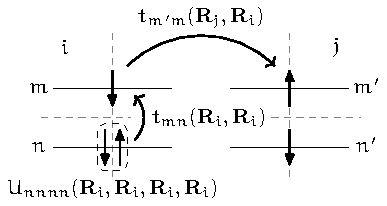
\includegraphics[width=.45\textwidth]{../../Graphics/Diagrams/two_orbitals_two_sites_hopping/two_orbitals_two_sites_hopping.pdf}
	\caption{Visual representation of a subset of interaction and hopping terms of \eqref{eq:general_hubbard_hamiltonian}. We show two lattice sites $i$ and $j$ with orbitals $m$, $n$ and $m'$, $n'$, respectively.}
	\label{fig:two_orbitals_two_sites_hopping}
\end{figure}
For brevity, the hopping matrix $t_{mm'}(\vv{R},\vv{R}')$ and Coulomb interaction $U_{lmm'l'}(\vv{R}_1,\vv{R}_2,\vv{R}_3,\vv{R}_4)$ are given by
\begin{align}
	t_{mm'}(\vv{R},\vv{R}')&=-\integral{}{}{^3r}w^*_{m\vv{R}}(\vv{r})\left [-\frac{\hbar^2}{2m}\nabla^2_{\vv{r}}+\mathcal{V}(\vv{r})\right ]w_{m'\vv{R}'}\quad\text{and}\\
	U_{lmm'l'}(\vv{R}_1,\vv{R}_2,\vv{R}_3,\vv{R}_4)&=\integral{}{}{^3r}\integral{}{}{^3r'}w^*_{l\vv{R}_1}(\vv{r})w^*_{m'\vv{R}_3}(\vv{r}')\frac{e^2}{|\vv{r}-\vv{r}'|}w_{l'\vv{R}_4}(\vv{r}')w_{m\vv{R}_2}(\vv{r}).\label{eq:wannier_interaction_real_space}
\end{align}
While for \eqref{eq:general_hubbard_hamiltonian} we have already restricted ourselves to a subspace of orbitals, it is still too complex to be solved exactly in the general case. The complexity can be further reduced by either placing further assumptions and restrictions or by using symmetries of the Hamiltonian, which are present in the hopping and interaction terms. Note, that \eqref{eq:wannier_interaction_real_space} overestimates the repulsive Coulomb interaction since screening effects from electrons outside the orbital subspace are not considered. One way to partly overcome this issue is proposed in the constrained Random Phase Approximation (cRPA). For details on how cRPA works, we refer the reader to \cite{crpa reference from somewhere}. 

\subsection{Fourier transform of the Coulomb term}

For reasons that become apparent later, it is more convenient to express the interaction term in Fourier space for diagrammatic calculations. The real-space interaction term in \eqref{eq:general_hubbard_hamiltonian} inherently depends on four lattice vectors. However, to simplify the notation, one of these arguments (e.g., $\vv{R}_4$) can be eliminated by expressing the distances relative to the lattice site $4$ rather than using their absolute positions. Therefore, 
\begin{align}
	\hat U=\frac 12 \sum_{\substack{\vv{R}_1\vv{R}_2\vv{R}_3\\ ll'mm'\\\sigma\sigma'}}U_{lmm'l'}(\vv{R}_1,\vv{R}_2,\vv{R}_3) \hat c^{\dagger}_{\vv{R}_1l\sigma} \hat c^{\dagger}_{\vv{R}_3 m'\sigma'} \hat c_{\vv{0}l'\sigma'} \hat c_{\vv{R}_2m\sigma}.\label{eq:hint_three_dependencies}
\end{align} 
This quantity naturally fulfils a swapping symmetry, where the simultaneous exchange of both incoming and outgoing particles keeps it invariant, i.e.,
\begin{align}
 	U_{lmm'l'}(\vv{R}_1,\vv{R}_2,\vv{R}_3)=U_{mll'm'}(\vv{R}_3-\vv{R}_2,-\vv{R}_2,\vv{R}_1-\vv{R}_2).
\end{align} 
The general Fourier transform of the tensor in \eqref{eq:hint_three_dependencies} with respect to the lattice positions $\vv{R}_i$ yields
\begin{align}
	U_{lmm'l'}^{\vv{qkk}'}=\sum_{\vv{R}_1\vv{R}_2\vv{R}_3} e^{i\vv{kR}_1}e^{-i(\vv{k}-\vv{q})\vv{R}_2}e^{-i(\vv{k}'-\vv{q})\vv{R}_3}U_{lmm'l'}(\vv{R}_1,\vv{R}_2,\vv{R}_3),
\end{align}
or for the full interaction operator in \eqref{eq:general_hubbard_hamiltonian}
\begin{align}
	\hat U=\frac 12 \sum_{\substack{\vv{qkk}'\\ ll'mm'\\\sigma\sigma'}}U_{lmm'l'}^{\vv{qkk}'}\hat c^{\dagger}_{\vv{k}l\sigma} \hat c^{\dagger}_{\vv{k}'-\vv{q} m'\sigma'} \hat c_{\vv{k}'l'\sigma'} \hat c_{\vv{k}-\vv{q}m\sigma},
\end{align}
where the Fourier transforms of the creation and annihilation operators are given by
\begin{align}
	\hat c^{(\dagger)}_{\vv{k}l\sigma}=\sum_{\vv{R}}e^{(-)i\vv{kR}}\hat c^{(\dagger)}_{\vv{R}l\sigma}.
\end{align}
One potential simplification to consider here is is neglecting orbital overlap of neighbouring sites, pairing up the operators at sites $\vv{0}$ and $\vv{R}$. This eliminates the $\vv{k}$-point dependence of the Coulomb operator and thus
\begin{align}
	U_{lmm'l'}&\equiv U_{lmm'l'}(\vv{0},\vv{0},\vv{0}),\quad\text{and}\\
	V^{\vv{q}}_{lmm'l'}&\equiv\sum_{\vv{R}\neq\vv{0}}e^{i\vv{qR}}U_{lmm'l'}(\vv{R},\vv{R},\vv{0}),
\end{align}
corresponding to a purely local interaction $U_{lmm'l'}$ and a purely non-local interaction $V^{\vv{q}}_{lmm'l'}$. In this case the exchange symmetry of the incoming and outgoing electron reduces to $U_{lmm'l'}=U_{mll'm'}$ and $V^{\vv{q}}_{lmm'l'}=V^{-\vv{q}}_{mll'm'}$.


\subsection{More symmetries, assumptions and the Kanamori-Hamiltonian}

cRPA is a framework in which all interaction combinations for $U_{lmm'l'}(\vv{R}_1,\vv{R}_2,\vv{R}_3,\vv{R}_4)$ can be computed, however there are certain symmetries and assumptions that help reduce the amount of individual elements of $U_{lmm'l'}(\vv{R}_1,\vv{R}_2,\vv{R}_3,\vv{R}_4)$ drastically. Similar simplifications can be made for the kinetic term in \eqref{eq:general_hubbard_hamiltonian}. Previously, it was stated that due to the localized nature of Wannier orbitals, the Hopping amplitudes reduce (rapidly) in magnitude the further the orbitals are located in real space due to reduced orbital overlap. The decay of $t_{mm'}(\vv{R},\vv{R}')$ is roughly proportional to $|\vv{R}-\vv{R}'|^{-1}$. Hence for practical calculations, a very good approximation can be achieved by considering only the three closest (in distance) hopping terms: nearest ($t$), next-nearest ($t'$); and next-next-nearest ($t''$) neighbor, see \figref{fig:hubbard_hopping} for an illustration. Elements of $U_{lmm'l'}(\vv{R}_1,\vv{R}_2,\vv{R}_3,\vv{R}_4)$ usually decay even faster than the hopping terms due to the integral over four orbitals in \eqref{eq:wannier_interaction_real_space} compared to two. Aside from this argument, further assumptions about the interaction can be made: (i) the Wannier functions respect SU(2) symmetry; (ii) the Wannier functions of the subset of orbitals preserve orbital symmetry; and (iii) the Coulomb interaction of electrons on different lattice sites is small compared to the on-site Coulomb interaction, e.g., $U_{lmm'l'}(\vv{R},\vv{R},\vv{R},\vv{R})\gg U_{lmm'l'}(\vv{R},\vv{R},\vv{R},\vv{R}')\gg U_{lmm'l'}(\vv{R},\vv{R},\vv{R}',\vv{R}'')$. Let us briefly justify these assumptions: (i) holds when spin-orbit coupling is ignored, the material is in the paramagnetic phase, and no external electromagnetic fields are applied \cite{georges hund}; (ii) applies to degenerate orbital subsets, like the $t_{2g}$ and $e_g$ orbitals in the $3d$ shell; and (iii) is valid as long as the Wannier functions remain localized around their respective lattice sites, which is generally true for $d$ or $f$ shells.

Under the assumptions (i)-(iii) $U_{lmm'l'}(\vv{R}_1,\vv{R}_2,\vv{R}_3,\vv{R}_4)$ is constrained to a single lattice site and has only three independent entries, commonly denoted by the intra-orbital and inter-orbital interactions $U$ and $U'$, respectively, and the Hund's exchange $J$ \cite{kanamori, georges hund coupling}. A visual representation of the effects of $U$, $U'$ and $J$ can be found in \figref{fig:kanamori_parameters_effects}.
\begin{figure}[ht!]
	\centering
	\begin{subfigure}[b]{.1\linewidth}
		\centering
		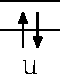
\includegraphics[page=1]{../../Graphics/Diagrams/kanamori_parameters_effects/kanamori_parameters_effects.pdf}
		\caption{\label{subfig:kanamori_parameter_effects_1}}
	\end{subfigure}\hfill
	\begin{subfigure}[b]{.1\linewidth}
		\centering
		\includegraphics[page=2]{../../Graphics/Diagrams/kanamori_parameters_effects/kanamori_parameters_effects.pdf}
		\caption{\label{subfig:kanamori_parameter_effects_2}}
	\end{subfigure}\hfill
	\begin{subfigure}[b]{.1\linewidth}
		\centering
		\includegraphics[page=3]{../../Graphics/Diagrams/kanamori_parameters_effects/kanamori_parameters_effects.pdf}
		\caption{\label{subfig:kanamori_parameter_effects_3}}
	\end{subfigure}\hfill
	\begin{subfigure}[b]{.2\linewidth}
		\centering
		\includegraphics[page=4]{../../Graphics/Diagrams/kanamori_parameters_effects/kanamori_parameters_effects.pdf}
		\caption{\label{subfig:kanamori_parameter_effects_4}}
	\end{subfigure}\hfill
	\begin{subfigure}[b]{.2\linewidth}
		\centering
		\includegraphics[page=5]{../../Graphics/Diagrams/kanamori_parameters_effects/kanamori_parameters_effects.pdf}
		\caption{\label{subfig:kanamori_parameter_effects_5}}
	\end{subfigure}
	\caption{Kanamori parameters $U$, $U'$ and $J$ as described in the text: \subref{subfig:kanamori_parameter_effects_1} intra-orbital Coulomb interaction, \subref{subfig:kanamori_parameter_effects_2}-\subref{subfig:kanamori_parameter_effects_3} inter-orbital Coulomb interaction, \subref{subfig:kanamori_parameter_effects_4} spin-flip of an electron pair and \subref{subfig:kanamori_parameter_effects_5} pair hopping.}
	\label{fig:kanamori_parameters_effects}
\end{figure}
These quantities are given by
\begin{align}
	U=U_{llll}&=\integral{}{}{^3r}\integral{}{}{^3r'}|w_l(\vv{r})|^2\mathcal{V}_c(\vv{r}-\vv{r}')|w_l(\vv{r}')|^2,\\
	U'=U_{llmm}&=\integral{}{}{^3r}\integral{}{}{^3r'}|w_l(\vv{r})|^2\mathcal{V}_c(\vv{r}-\vv{r}')|w_m(\vv{r}')|^2\quad\text{and}\\
	J=U_{lmml}&=\integral{}{}{^3r}\integral{}{}{^3r'} w^*_l(\vv{r})w^*_m(\vv{r}')\mathcal{V}_c(\vv{r}-\vv{r}') w_l(\vv{r}')w_m(\vv{r}),
\end{align}
where $\mathcal{V}_c(\vv{r}-\vv{r}')$ is the screened Coulomb interaction term. For cubic symmetry - due to constraint (ii) - there are only two independent quantities in the interaction, resulting in $U'=U-2J$. With the help of these three parameters we can simplify the Hamiltonian of \eqref{eq:general_hubbard_hamiltonian} and for the general case the so-called Kanamori-Hamiltonian \cite{kanamori, georges hund coupling} reads
\begin{align*}
	\mathcal{H}_{\text{Kanamori}}&=-\sum_{\substack{\vv{R}\vv{R}'\\ mm',\sigma}}t_{mm'}(\vv{R},\vv{R}')\hat c^{\dagger}_{\vv{R}m\sigma}\hat c_{\vv{R}'m'\sigma}\\
	&\qquad +U\sum_{\vv{R},l} \hat n_{\vv{R}l\uparrow}\hat n_{\vv{R}l\downarrow}+\sum_{\substack{\vv{R},l\neq m\\\sigma\sigma'}}(U'-J\delta_{\sigma\sigma'}) \hat n_{\vv{R}l\sigma} \hat n_{\vv{R}m\sigma'}\\
	&\qquad -J\sum_{\vv{R},l\neq m}\hat c^\dagger_{\vv{R}l\uparrow}\hat c_{\vv{R}l\downarrow}\hat c^\dagger_{\vv{R}m\downarrow}\hat c_{\vv{R}m\uparrow}+J\sum_{\vv{R},l\neq m}\hat c^\dagger_{\vv{R}l\uparrow}\hat c^\dagger_{\vv{R}l\downarrow}\hat c_{\vv{R}m\downarrow}\hat c_{\vv{R}m\uparrow}\numberthis,
\end{align*}
where $\hat n_{l\sigma}$ is the number operator ($\hat c^\dagger_{l\sigma}\hat c_{l\sigma}$) that counts the number of electrons in orbital $l$ with spin $\sigma$. The Kanamori Hamiltonian is a widely used model for strongly correlated systems and it can capture a lot of physics despite its rather crude approximations. Today, the Kanamori Hamiltonian is mostly used not only to describe spin and orbital order, including magnetically ordered phases in materials with partially filled $d$ or $f$ shells, but also to capture a variety of Mott-insulating states, where strong on-site electron repulsion causes electron localization.

\section{The single-band Hubbard Hamiltonian}

The most widely used model Hamiltonian to describe strongly correlated materials is the one-band Hubbard model. It is the single-orbital version of the Kanamori Hamiltonian and reads
\begin{align}\label{eq:one_band_hubbard_model}
	\mathcal{H}_{\text{Hubbard}}=-\sum_{i\neq j,\sigma}t_{ij}\hat c^{\dagger}_{i\sigma} \hat c_{j\sigma}+U\sum_{i}\hat n_{i\uparrow}\hat n_{i\downarrow}-\mu \sum_{i}(\hat n_{j\uparrow}+\hat n_{j\downarrow}),
\end{align}
where $i$ and $j$ denote the lattice site in the $N$-dimensional lattice and the hopping is spin-independent. The interaction $U$ is purely local and $\mu=t_{ii}$ is the chemical potential. Due to the reduction to a single orbital, the interaction terms $U'$ and $J$ do not exist any more as they used to incorporate different orbitals. 
\begin{figure}[ht!]
	\centering
	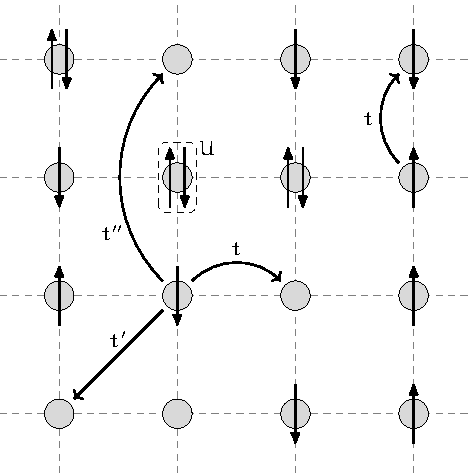
\includegraphics[width=.5\textwidth]{../../Graphics/Diagrams/single_band_hubbard_model/single_band_hubbard_model.pdf}
	\caption{Visual representation of the two-dimensional square lattice Hubbard model. Each lattice site either contains zero, one or two electrons. Every circle represents a local orbital at any site. Here, $t$, $t'$ and $t''$ denote nearest-neighbour hopping, next-nearest-neighbour hopping and next-next-nearest-neighbour hopping, respectively. Reasonable values for $t$, $t'$, $t''$ and $U$ are obtained from density functional theory (DFT) calculations \cite{PavariniE2001BTiH} or extracted from ARPES studies \cite{HashimotoM2008Deot}. For e.g., cuprates, one finds that $t\approx$ 0.3-0.5~eV, $t'\approx$ -0.2$t$, $t''\approx$ 0.1$t$ and $U\approx$ 8$t$.}
	\label{fig:hubbard_hopping}
\end{figure}

This is one of the simplest forms of the most general Hubbard Hamiltonian of \eqref{eq:general_hubbard_hamiltonian}, however it can still not be solved exactly since the kinetic term is diagonal in momentum space whereas the interaction term is diagonal in real space. A general analytical solution to the model does therefore not exist, however recent advances allowed numerical calculations to exactly calculate the eigendecomposition of the Hubbard Hamiltonian for a couple different parameter sets. To visually illustrate the model's description, a representation of the hopping and interaction terms of \eqref{eq:one_band_hubbard_model} can be seen in \figref{fig:hubbard_hopping}.
\\
The very extreme simplification of the Hubbard model is called the Hubbard Atom and it represents an isolated lattice site with either zero, one or two electrons occupying a single orbital interacting through the instantaneous electrostatic repulsion $U$. It is also often coined \say{atomic limit}, because it can be formulated as a limiting case for the Hubbard model where all hopping amplitudes are set to zero. The Hubbard Atom is analytically solvable and can already give a lot of information about non-perturbative processes in condensed matter physics.
\\

In the last chapter, we looked at the fundamental Hamiltonians and a few specific models that create the theoretical foundation for modelling strongly correlated electron systems, such as transition metal oxides (e.g., manganites, cuprates or nickelates), heavy fermion systems (e.g., compounds containing rare-earth or actinide elements), Mott insulators (e.g., $\text{V}_2\text{O}_3$) and many more. We have developed the fundamental ideas required to explain the distinctive behaviour of particles in systems where interactions play an important role.

With this framework in place, we now proceed to introduce the mathematical tools required to perform calculations within these models. The next two chapters present a detailed toolkit, including many-body Green's functions and diagrammatic methods, such as dynamical mean-field theory (DMFT) or the dynamical vertex approximation ($\text{D}\Gamma\text{A}$). These approaches ready us to translate the abstract models into concrete results, allowing for the computation of observables and the quantitative study of strongly correlated systems. This toolkit will be essential for extracting physical insights from the models we have discussed and for bridging theory with experimental observations in the field.

\end{document}
